\titledquestion{MCTS practice}
In a Monte Carlo Tree, each node represents a state. In a node, using $a/b$ to represent its historical information, which means this state won $a$ times in $b$ times of search. In this problem, we use $UCB = \frac{a_i}{b_i} + \sqrt{\frac{\log_2(a_p)}{b_i}}$ , where node $p$ is the parent node of node $i$.
\newline
Here is a part of a Monte Carlo Tree, containing the first three layers (i.e. the fourth and deeper layers are omitted).

\begin{center}
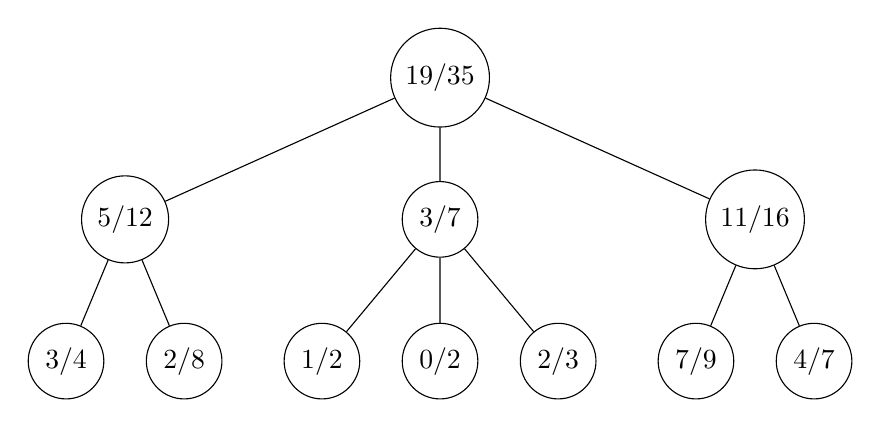
\begin{tikzpicture}[level distance=1.8cm,
            level 1/.style={sibling distance=4cm},
            level 2/.style={sibling distance=1.5cm},
            level 3/.style={sibling distance=1.5cm},
            every node/.style = {draw, circle}]
\node {$19/35$}
    child {node {$5/12$}
        child {node {3/4}}
        child {node {2/8}}
    }
    child {node {$3/7$}
        child {node {$1/2$}}
        child {node {$0/2$}}
        child {node {$2/3$}}
    }
    child {node {$11/16$}
        child {node {$7/9$}}
        child {node {$4/7$}}
    };

\end{tikzpicture}
\end{center}

\begin{parts}

\part[2] Given a Monte Carlo Tree above, which node in the third layer will be selected according to the MCTS algorithm?

\begin{choices}
    \choice $3/4$
    \choice $2/8$
    \choice $1/2$
    \choice $0/2$
    \choice $2/3$
    \choice $7/9$
    \choice $4/7$
\end{choices}

\part[4] After selecting a leaf node (deeper than the third layer), in the simulation step, the algorithm performs 5 simulations and wins 3 times. Please draw the new Monte Carlo Tree (the first three layers) after the Backpropagation step.

\begin{solution}
    \vspace{2in}
\end{solution}

\end{parts}
